
\subsubsection{Using two beams at a time}
Having experimentally determined the V2PM and inverted it to obtain the P2VM, the object visibility and phase are retrieved from the experimental  data. First using the same set of data used to calibrate the V2PM and then using new ones to test the reproducibility of the method. 

The results of the retrieved phases from the data used to calibrate the V2PM matrix are shown on Fig.\ref{fig:retrieved_visi_expe}. These results aren't biased by the calibration of the V2PM because the V2PM only take into account of the visibility and phase of the output interferogram at the position of their maximum. What is flagrant from these results and the simulated ones on a similar component (see \ref{an:retriev}) is that experimentally the retrieved visibility tend to oscillate a lot more around the theoretical one (expecially for baseline 14. These oscillations are mostly due to the highly overlapping output signal (as explained in the first chapter) and the delay-line being not verry accurate thus changing the coupling a little from one measurement to the other (this will be verified further). Contributions of the noise are also not negligible. With all of these imperfections the retrieve visibility are around the zone of interest (around the maximum) accurate at 10\% for the best baselines to 20\% for the worst. The visibilities retrieved on the second dataset recorded right after the calibration of the V2PM are presented on figure \ref{fig:retrieved_visi_expe2} and are far from as good as the first ones. This is mostly because of the delay-line altering the coupling in their movement and is especially visible on the retrieved visibility for baseline 1-2, 1-3 and 1-4 which were recorded in the same order moving the delay-line of input 1.  


\begin{figure}[htbp!]
 \centering
 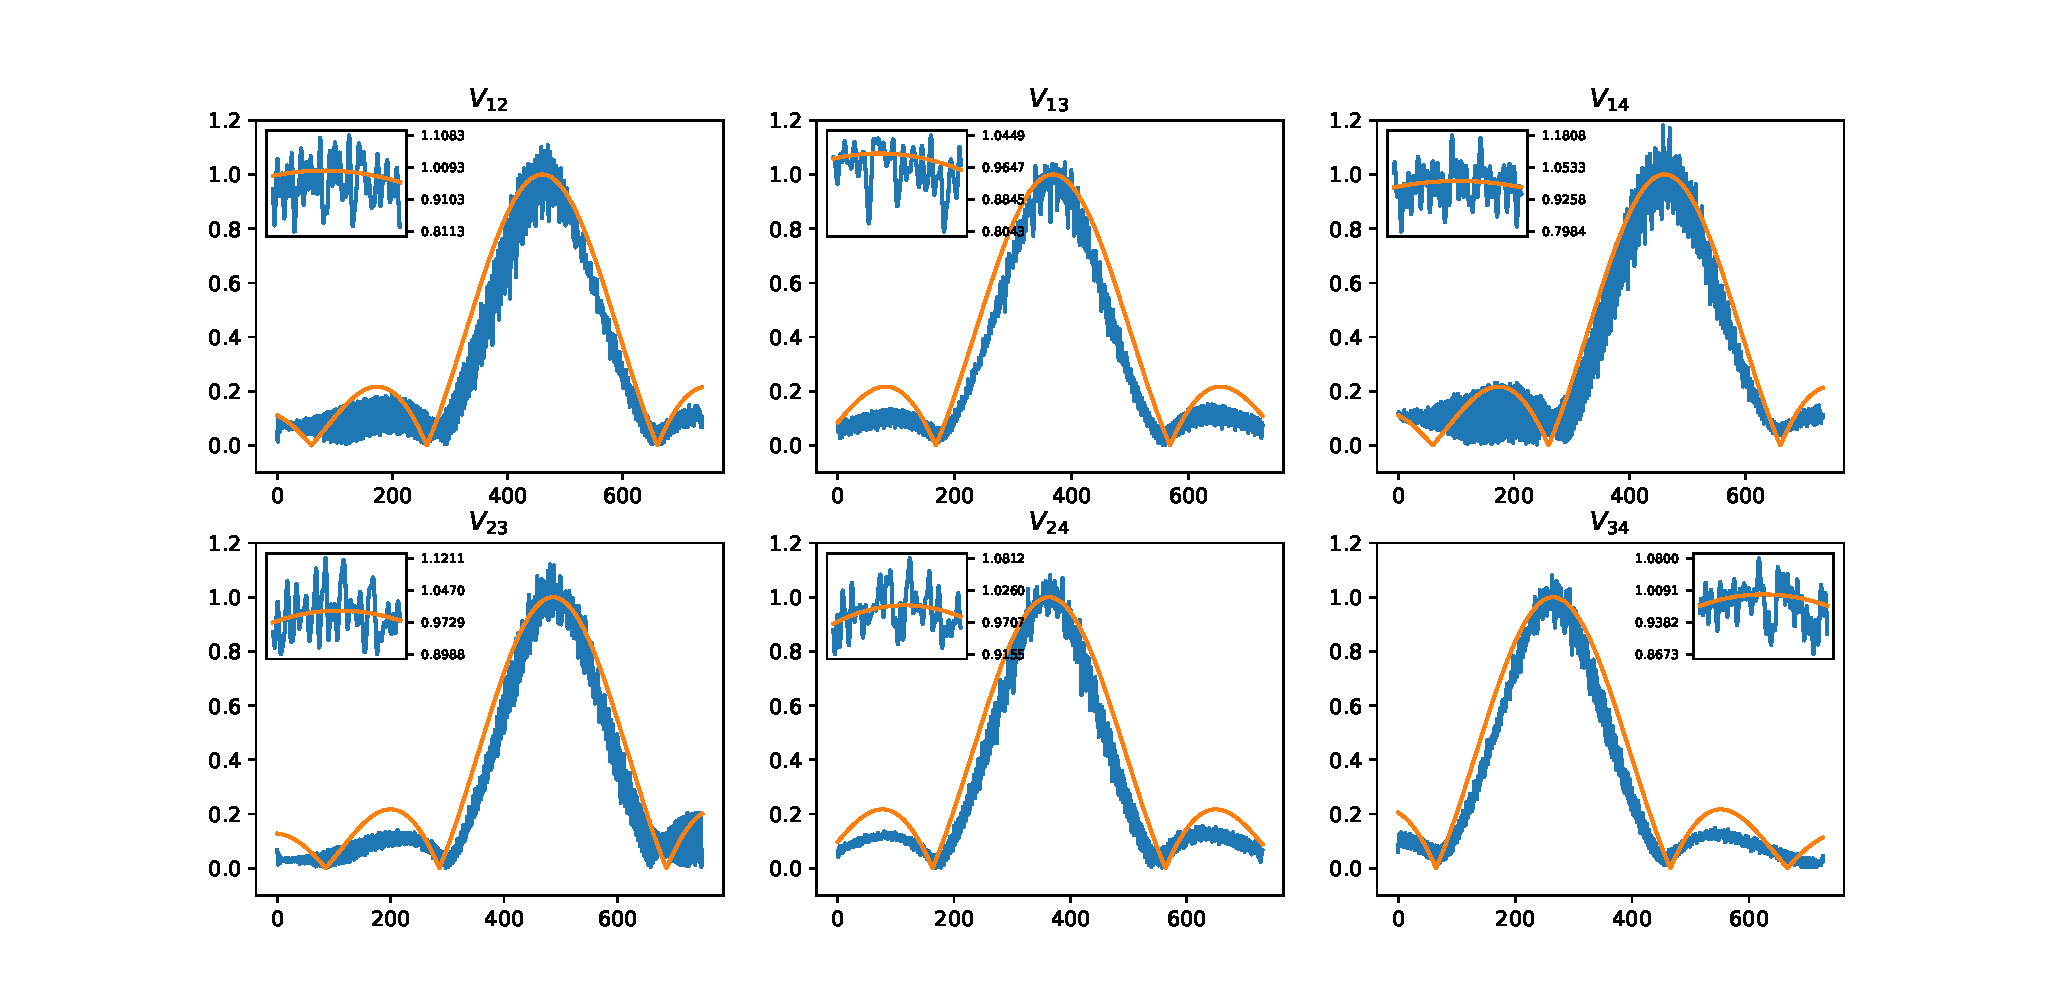
\includegraphics[scale=.4]{../picture/retrieve_visi_expe.pdf}
 \caption{Experimentally retrieved visibility from the dataset used to calibrate the V2PM. Baselines numbering 1, 2, 3, 4 refers to the input waveguides (respectively  9, 14, 10 and 19).The x-axis is the OPD in µm and the y-axis the visibility. The blue line is the actual retrieved data and the orange line the theoretical result. The inset is a zoom of the 50µm opd around the maximum. }
 \label{fig:retrieved_visi_expe}
\end{figure}

\begin{figure}[htbp!]
 \centering
 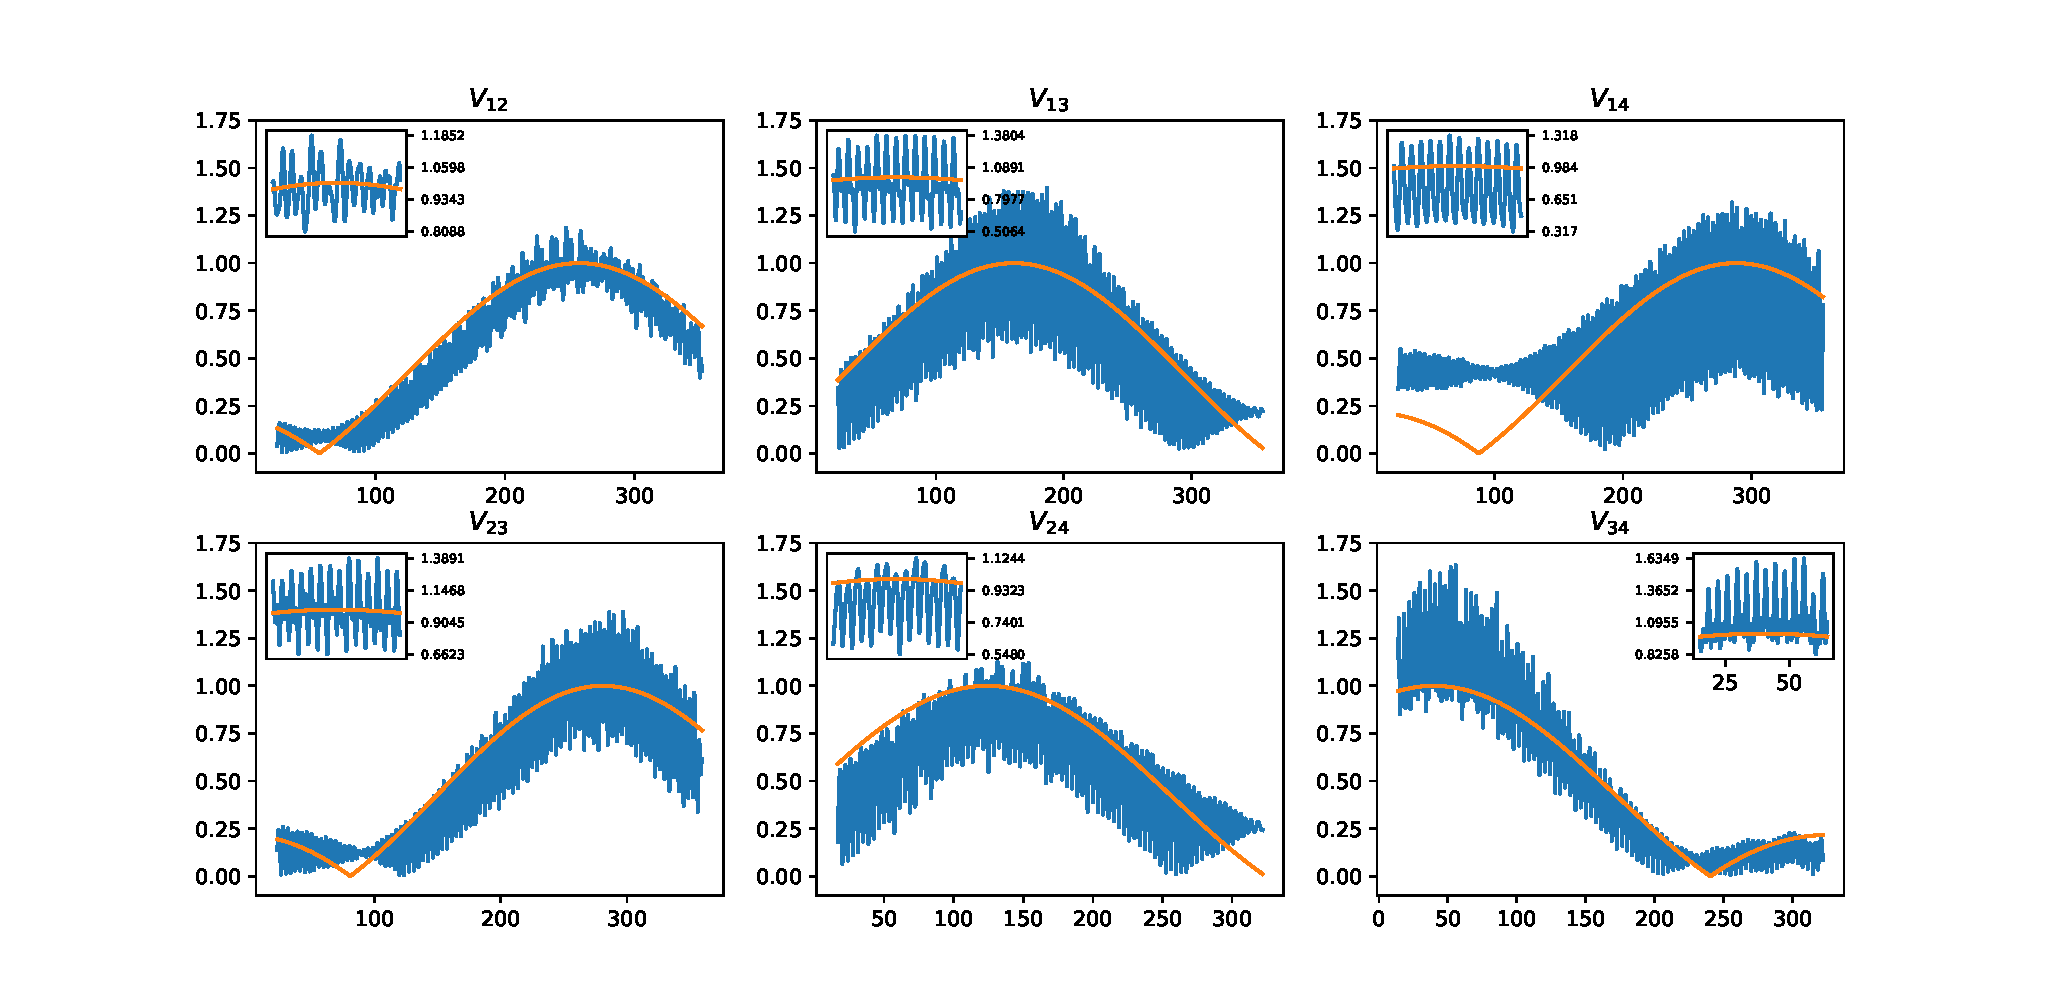
\includegraphics[scale=.4]{../picture/retrieve_visi_expe2.pdf}
 \caption{Experimentally retrieved visibility from the data recorded after the V2PM calibration. Baselines numbering 1, 2, 3, 4 refers to the input waveguides (respectively  9, 14, 10 and 19).The x-axis is the OPD in µm and the y-axis the visibility. The blue line is the actual retrieved data and the orange line the theoretical result. The inset is a zoom of the 50µm opd around the maximum. }
 \label{fig:retrieved_visi_expe2}
\end{figure}

Concerning the retrieved phase, the results are presented in Fig\ref{fig:retrieved_phase_expe} for the dataset used to calibrate the V2PM and Fig.\ref{retrieve_phase_expe2} for the second dataset zoomed around the maximum of the interferogram (the "0" OPD). Comparison with the simulated one on the optimised component at 3.4µm and bandwidth 70nm can be done using Appendix \ref{an:retriev}. It appear that the results are better on the second set of data recorded than on the one used to calibrate the V2PM. This suggest that the phase retrieval is less sensitive to the inperfections of the delay-line and that the uncertainties on it's retrieval are more intrinsic to the noise and the "apparent wavelength" explained before. In all case the residues show a standard deviation to 0 ranging from 0.08 to 0.4 rad. This is equivalent to a sensitivity from $\frac{\lambda_0}{9}$ to $\frac{\lambda_0}{46}$ depending on the baseline and the quality of the calibration ($lambda_0$ being the mid-range wavelength thus 3.745µm). In the simulated case with the optimised component (70nm bandwidth centered on 3.4µm wavelength) the residue was about 0.086 rad for all baselines suggesting a possible accuracy of $\frac{\lambda_0}{40}$ for all baselines. To compare Diener et al. presented retrieved visibility ranging from $0.96\pm0.04$ to $1.04\pm0.06$ and phases residue ranging from 0.13 to 0.18 rad in\cite{Diener2017} using a similar component with monochromatic light at 3.39µm.  

\begin{figure}[htbp!]
 \centering
 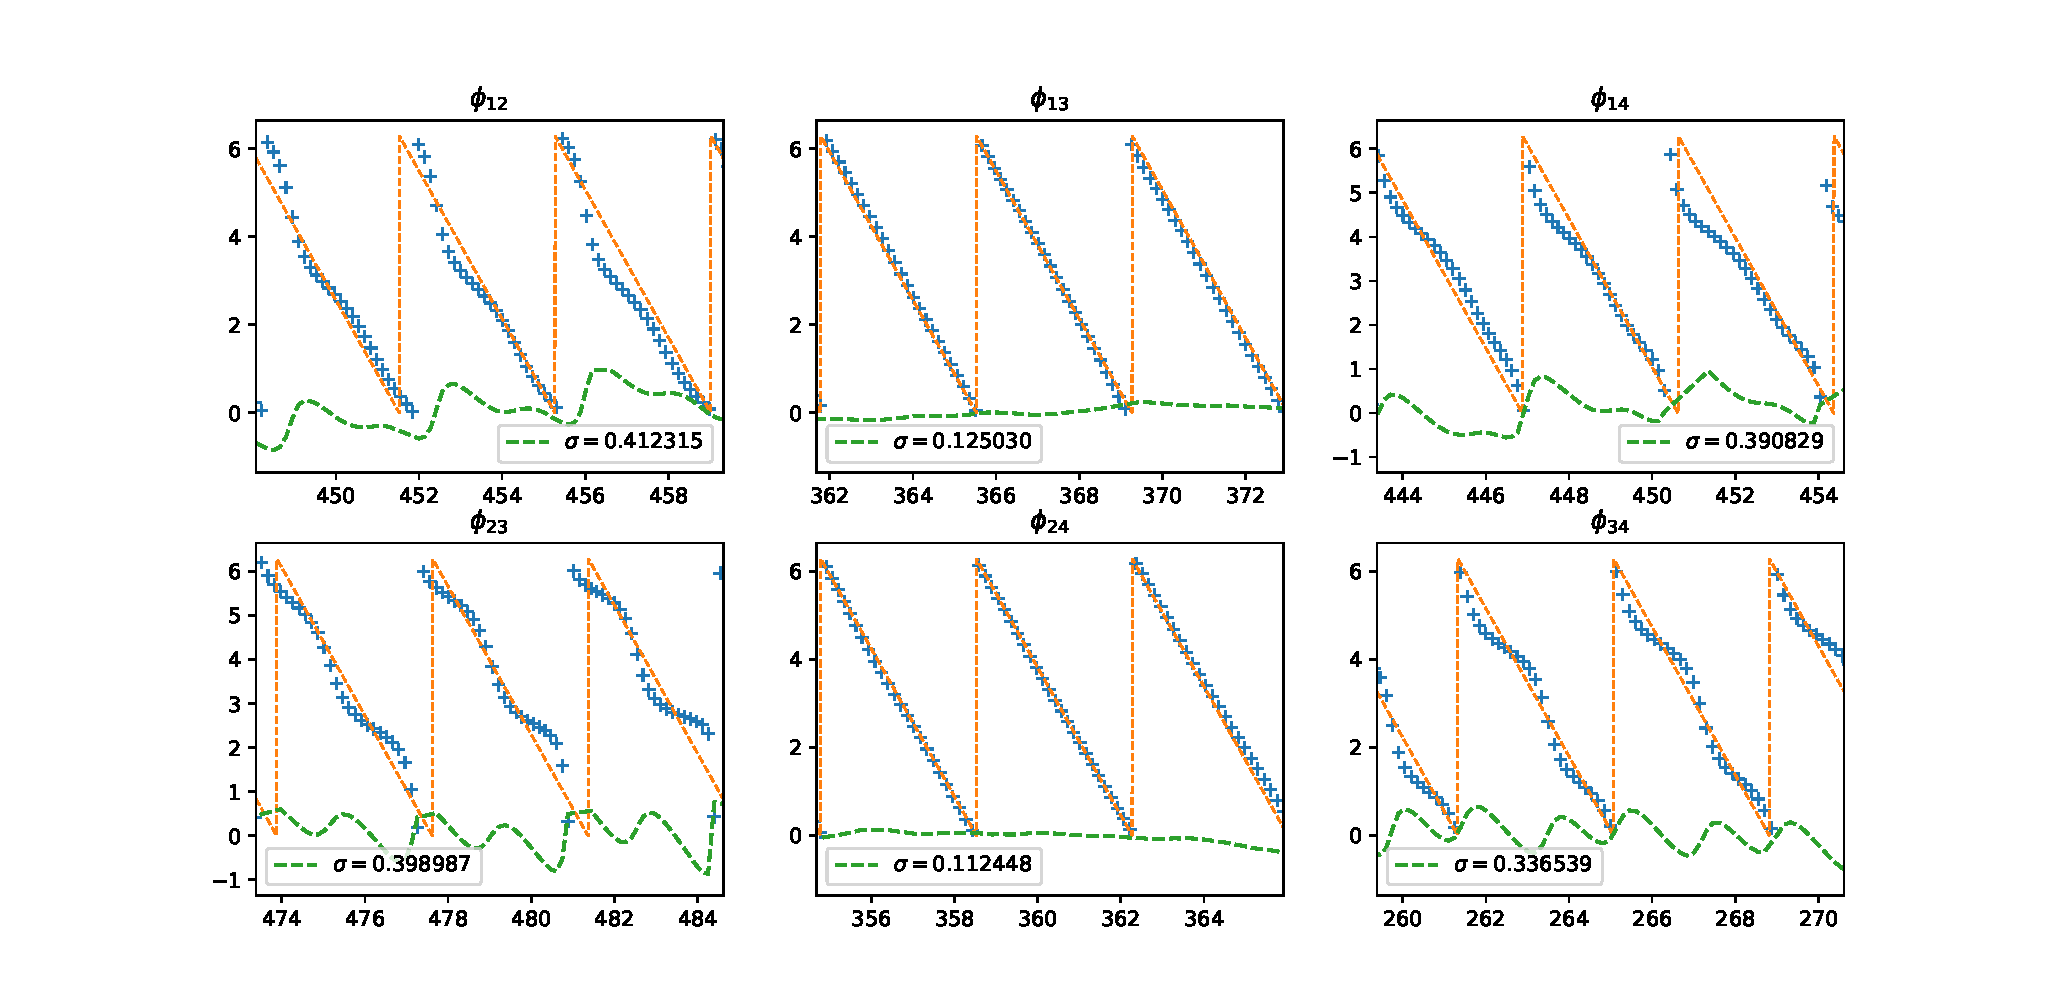
\includegraphics[scale=.4]{../picture/retrieve_phase_expe1.pdf}
 \caption{Experimentally retrieved phase from the dataset used to calibrate the V2PM. Baselines numbering 1, 2, 3, 4 refers to the input waveguides (respectively  9, 14, 10 and 19). The blue line is the actual retrieved data, the orange line the theoretical result and the green line the residues (difference between the blue and orange one). $\sigma$ is the standard deviation of the residues in rad. The x-axis is the OPD in µm and the y-axis the phase in rad. }
 \label{fig:retrieved_phase_expe}
\end{figure}

\begin{figure}[htbp!]
 \centering
 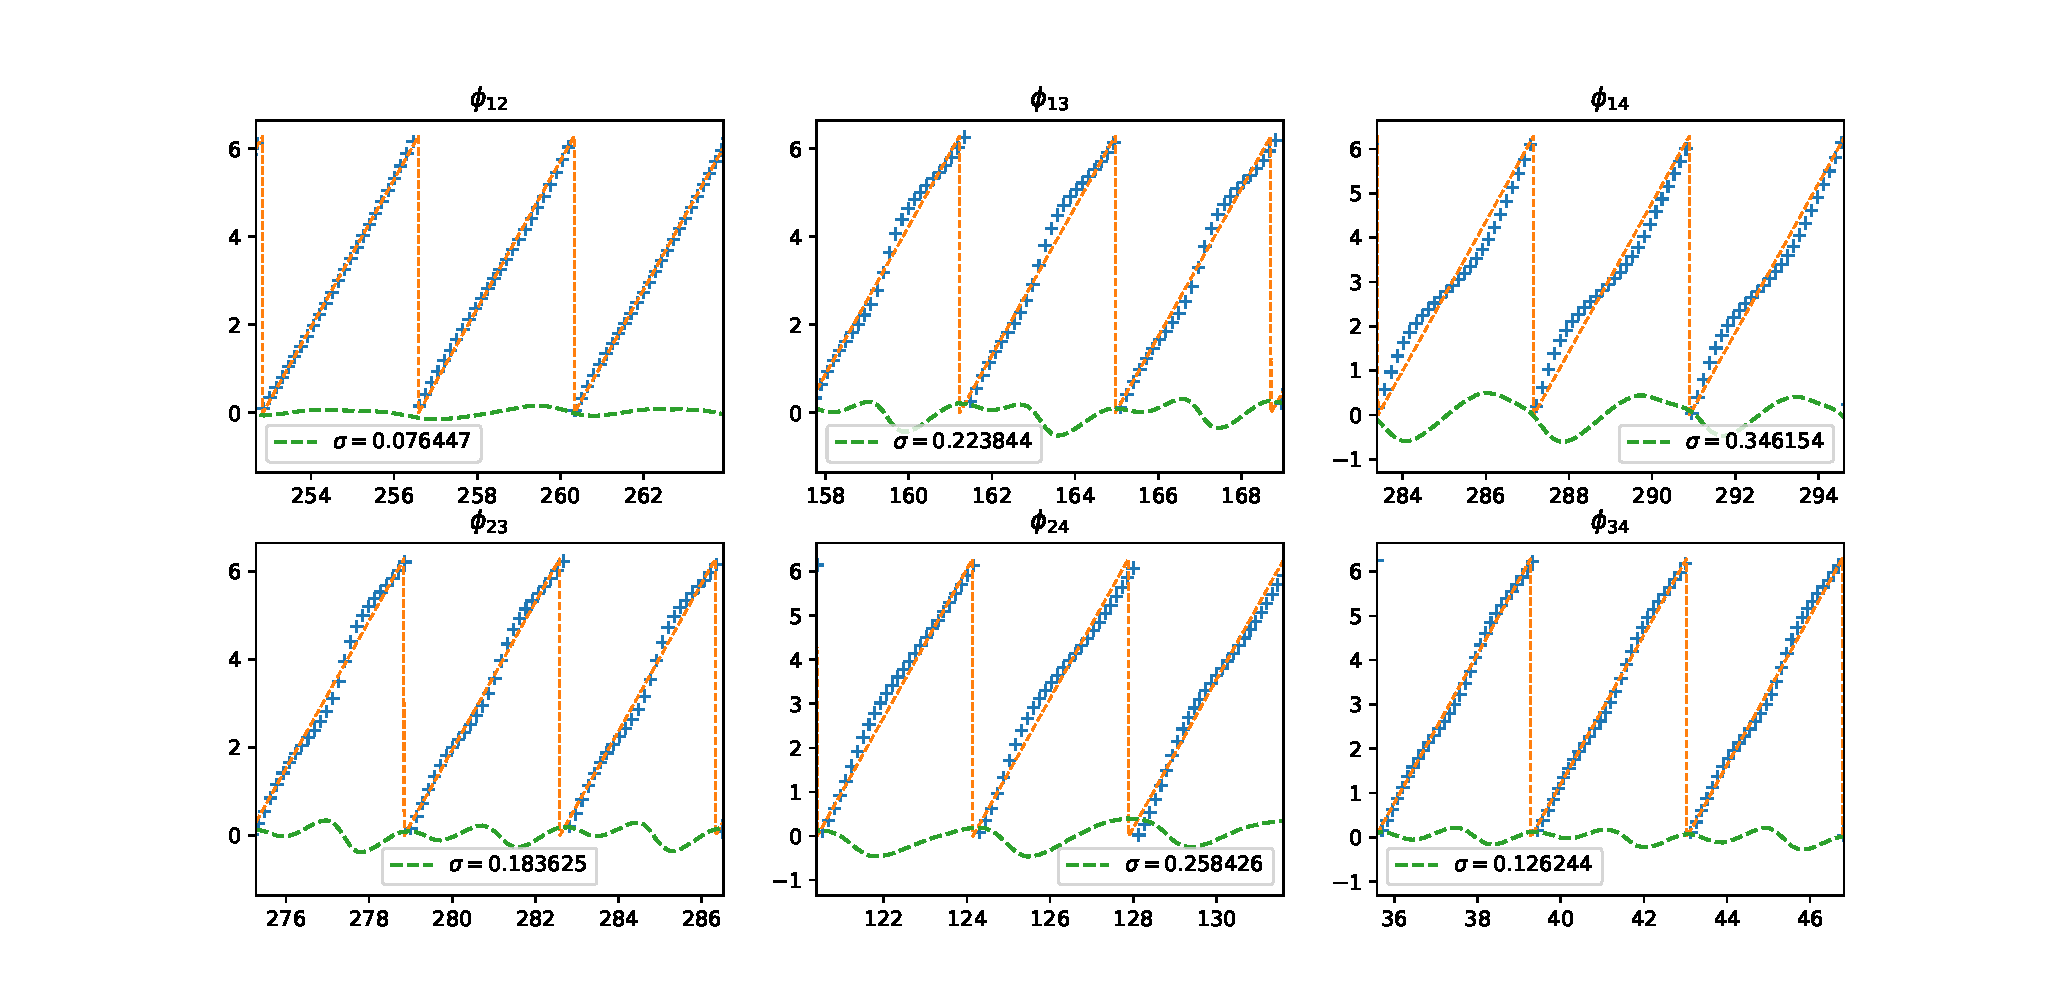
\includegraphics[scale=.4]{../picture/retrieve_phase_expe2.pdf}
 \caption{Experimentally retrieved phase from the data recorded after the V2PM calibration. Baselines numbering 1, 2, 3, 4 refers to the input waveguides (respectively  9, 14, 10 and 19). The blue line is the actual retrieved data, the orange line the theoretical result and the green line the residues (difference between the blue and orange one). $\sigma$ is the standard deviation of the residues in rad. The x-axis is the OPD in µm and the y-axis the phase in rad. }
 \label{fig:retrieved_phase_expe2}
\end{figure}

For now the experimental demonstration of the feasibility and usability of the Zig-Zag DBC has been done using it to combine only 2 beams at a time. The final purpose of this component beeing to combine 4 telescopes one experimental measurement has been done using the 4 beams.

\subsubsection{Combining the 4 beams}
In order demonstrate the usability of the Zig-Zag DBC to combine 4 telescopes at a time the 4 beams where coupled into the component and the P2VM applied to the measured data to retrieve the phases and visibilities of the source. Because of the Delay-line being not very reproducible in its mouvement only the one that moved the less were used for this measurement (corresponding to input 3, WG 10). The results are sown on Fig.\ref{fig:retrieved_visi_4BL2} and Fig.\ref{fig:retrieved_phase_4BL2}. Only the delay-line of input 3 is scanned thus the visibility and phase of BL 1-2, 1-4 and 2-4 are expected to be constant. The visibility and phase of BL 1-3, 2-3 and 3-4 are supposed to look like the ones of Fig\ref{fig:retrieved_visi_expe}  and Fig.\ref{fig:retrieved_phase_expe2} respectively. Once again the retrieving algorythm seems to be more accurate on retrieving the phases than the visibilities. This can be explained by the fact that to retrieve the visibilities, 4 different component of the vector $\vec{V}$ are used opposed to 2 to retrieve the phase (see Eq.\ref{eq:banana}) making the phase less sensitive to errors.

Concerning the phase of the 3 scanned baselines, the standard deviation of the residue is less than 0.16 rad which is better than in some case using only 2 beams and the same order of magnitude than reported in \cite{Diener2017}. This can be explain by more amplitude in the interferograms  resulting to higher SNR. The phase of the non scanned baselines shows more volatility (for BLs 1-2 and 1-4 especially). 

Concerning the visibilities of the 3 scanned baselines, the shapped of the cardinal sine is visible and the maximum around 1 but the 

\begin{figure}[htbp!]
 \centering
 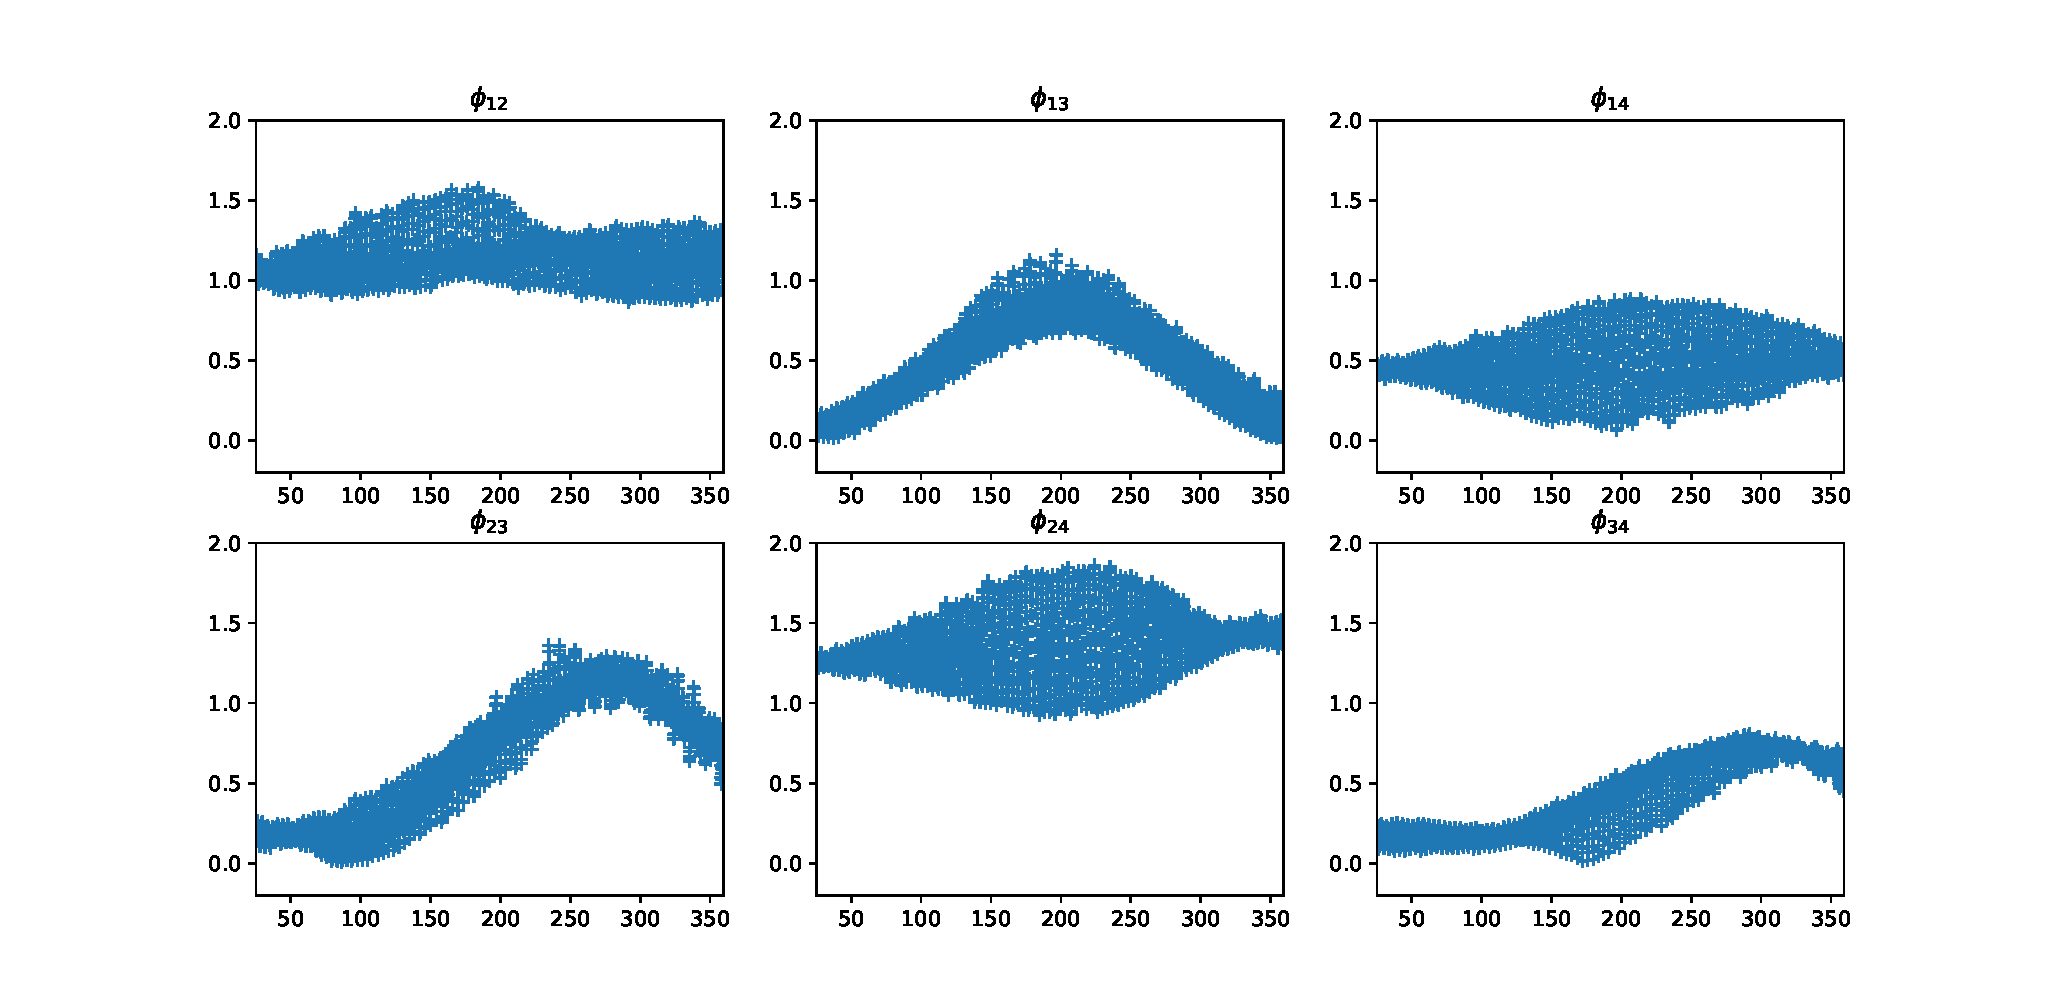
\includegraphics[scale=.4]{../picture/retrieve_visi_4BL2.pdf}
 \caption{Experimentally retrieved visibility from the data recorded after the V2PM calibration. Baselines numbering 1, 2, 3, 4 refers to the input waveguides (respectively  9, 14, 10 and 19). The x-axis is the OPD in µm and the y-axis the phase in rad. }
 \label{fig:retrieved_visi_4BL2}
\end{figure}

\begin{figure}[htbp!]
 \centering
 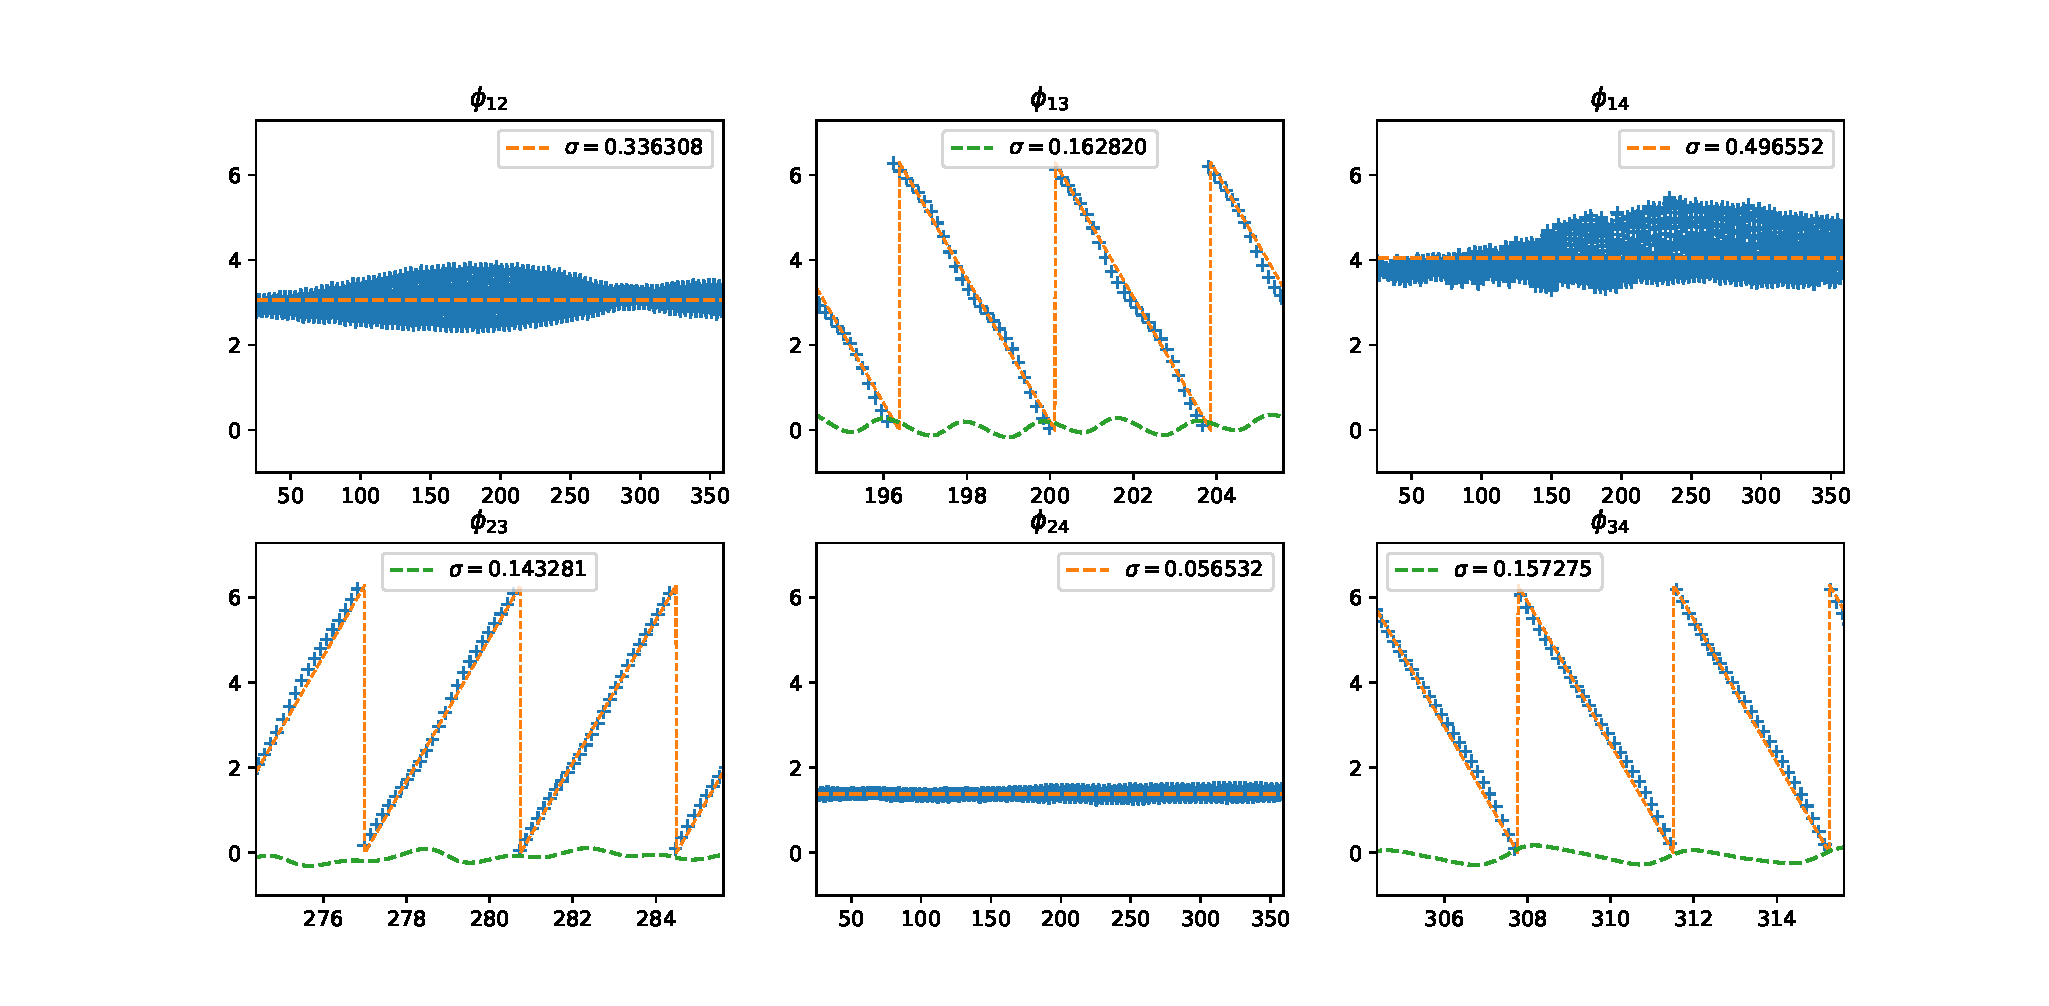
\includegraphics[scale=.4]{../picture/retrieve_phase_4BL2.pdf}
 \caption{Experimentally retrieved phase from the data recorded after the V2PM calibration. Baselines numbering 1, 2, 3, 4 refers to the input waveguides (respectively  9, 14, 10 and 19). The blue line is the actual retrieved data, the orange line the theoretical result and the green line the residues (difference between the blue and orange one). $\sigma$ is the standard deviation of the residues in rad. The x-axis is the OPD in µm and the y-axis the phase in rad. }
 \label{fig:retrieved_phase_4BL2}
\end{figure}

The retrieval of the phase and visibility a source using the ZigZag-DBC have been demonstrated to be as accurate using a broad-band source of 70nm with similar degree of accuracy than using monochromatic light as reported in \cite{Diener2017} using 2 beams at a time. In the case of using 4 beams the method used showed lower accuracy on retrieving the visibilities. We are convinced that the variation of the coupling due to the delay-lines being not very accurate contributed a lot to the errors and we are convinced that better results could be obtained with better delay-lines (as the simulations showed far better accuracy).   
